\PassOptionsToPackage{dvipsnames}{xcolor}

\documentclass[11pt]{article}
\usepackage{epsfig,endnotes,cite}
\usepackage{fullpage}
\usepackage{times}

\date{}

\newcommand{\todo}[1]{\noindent\textcolor{red}{[TODO: #1]}}
\newcommand{\htor}[1]{\noindent\textcolor{green}{[htor: #1]}}

% Copyright
%\setcopyright{none}
%\setcopyright{acmcopyright}
%\setcopyright{acmlicensed}
%\setcopyright{rightsretained}
%\setcopyright{usgov}
%\setcopyright{usgovmixed}
%\setcopyright{cagov}
%\setcopyright{cagovmixed}


\usepackage{amsmath,amssymb}
\usepackage{footnote}
\usepackage[hidelinks]{hyperref}

\usepackage{booktabs}
\usepackage{subcaption}
\usepackage{listings}
\usepackage{amsthm}
\usepackage{bm}
\lstset{
	numbers=left, 
	numberstyle=\tiny, 
	numbersep=2pt, 
	frame = single, 
	language=C++,
	basicstyle=\tiny\ttfamily,
	keywordstyle=\color{blue}\ttfamily,
	stringstyle=\color{red}\ttfamily,
	commentstyle=\color{Green}\ttfamily,
	breaklines=true,
	tabsize=2,
	framexleftmargin=5pt
	}
\usepackage{enumitem}
\setitemize{noitemsep,topsep=0pt,parsep=0pt,partopsep=0pt}

\usepackage{tikz}
\usepackage{enumitem}
\usepackage{multirow}
\usetikzlibrary{positioning, fit, shapes, patterns, calc}

\usepackage[parfill]{parskip}

\renewcommand{\paragraph}[1]{\vspace{0.1em} \noindent \textbf{#1}}

\newtheorem{theorem}{Theorem}[section]
\newtheorem{corollary}{Corollary}[theorem]
\newtheorem{lemma}[theorem]{Lemma}
\newtheorem{remark}[theorem]{Remark}


\newcommand{\mml}{$\textsc{SparCML}$}

\begin{document}
\title{\mml{}: High-Performance Sparse Communication \\ for Machine Learning}

\author{
{\rm C\'edric Renggli}\\
ETH Zurich
\and
{\rm Dan Alistarh}\\
IST Austria
\and 
{\rm Torsten Hoefler}\\
ETH Zurich
\and 
{\rm Mehdi Aghagolzadeh}\\
Microsoft
% copy the following lines to add more authors
% \and
% {\rm Name}\\
%Name Institution
} % end author


%\authorinfo{Cedric Renggli}{ETH Zurich}{}
%\authorinfo{Dan Alistarh}{IST Austria}{}
%\authorinfo{Torsten Hoefler}{ETH Zurich}{}

\maketitle

\begin{abstract}
	\noindent
	One of the main drivers behind the rapid recent advances in machine
	learning has been the availability of efficient system support. 
	%
	%This comes both through faster hardware, but also in the form of
	%efficient software frameworks and programming models.
	%
	Despite existing progress, scaling compute-intensive machine learning
	workloads to a large number of compute nodes is still a challenging
	task. 
	%
	In this paper, we address this challenge, by proposing
	\mml{},\footnote{Stands for Sparse Communication layer for Machine
		Learning, to be read as \emph{sparse ML}.} a general, scalable
	communication layer for machine learning applications. 
	%
	\mml{} is built on the observation that many distributed machine
	learning algorithms either have naturally sparse communication
	patterns, or have updates which can be sparsified in a structured way
	for improved performance, without loss of convergence or accuracy.  
	%
	To exploit this insight, we analyze, design, and implement a set of
	communication-efficient protocols for sparse input data, in
	conjunction with efficient machine learning algorithms which can
	leverage these primitives. 
	%
	Our communication protocols generalize standard collective operations,
	by allowing processes to contribute sparse input data vectors, of
	\emph{heterogeneous sizes}. 
	%
	%We call these operations \emph{collectives on sparse streams}, and
	%present efficient practical algorithms with strong theoretical bounds
	%on their running time and communication cost. 
	%
	Our generic communication layer is enriched with additional features,
	such as support for non-blocking (asynchronous) operations and support
	for low-precision data representations. 
	%
	We validate our algorithmic results experimentally on a range of
	large-scale machine learning applications and target architectures,
	showing that we can leverage sparsity for order-of-magnitude runtime
	savings, compared to existing methods and frameworks. 
\end{abstract}

\maketitle

\section{Introduction and Motivation}

A key enabling factor behind the recent progress in machine learning has been \emph{efficient system support}, in the form of efficient hardware, e.g.~\cite{TPU}, but also via specialized \emph{software platforms}, e.g.~\cite{TF, CNTK, MXNET}. 
Due to the sheer size of the datasets and models, production-scale machine learning workloads are usually \emph{distributed} across multiple computing nodes, such as  clusters of CPUs or GPUs in a datacenter environment. 
The arguably standard distribution strategy in machine learning is \emph{data parallelism}, in which nodes partition the dataset, and maintain consistent copies of the set of model parameters by exchanging messages, either all-to-all, or through a coordinator node, called a parameter server~\cite{PS}.  
The high \emph{bandwidth} and \emph{latency} requirements of these workloads put pressure on system scalability. 
For example, when training a deep neural network such as AlexNet~\cite{AlexNet} through stochastic gradient descent (SGD), nodes perform \emph{all-to-all} exchanges of their gradient updates upon every batch of examples: the message size per node is $>200$ MB, exchanged every few milliseconds. This communication can easily become the system bottleneck. 

Given the significant impact of communication, significant effort has been invested into identifying scalable solutions. Virtually all major frameworks  optimize for efficient communication~\cite{CNTK, seide20141, TF, MXNET, PyTorch}, while GPU vendors are developing specific communication layers for this goal~\cite{NCCL}. 
The research community proposed several communication-reduction techniques, such as \emph{quantization}~\cite{seide20141, alistarh2016qsgd}, \emph{asynchronous communication}~\cite{zhang2017yellowfin},  \emph{structured sparsification}~\cite{aji2017sparse, dryden2016communication, sun2017meprop}, or \emph{large batch methods}~\cite{goyal2017accurate, you2017scaling}. However, scaling machine learning applications remains a complex process, requiring non-trivial insights. 

\paragraph{Conceptual Contribution.} We propose \mml{}, a scalable, general communication layer for machine learning. 
\mml{} starts from the idea that, to reduce communication and synchronization cost, we can exploit the \emph{relaxed consistency} supported by machine learning applications. 
In particular, individual nodes can compute with an \emph{inconsistent} view of the set of model parameters, which can be corrupted with noise from various sources, such as communication quantization or asynchrony. 
The immediate system implication, which we exploit in \mml{}, is that the updates which nodes wish to communicate are either \emph{naturally sparse}~\cite{webb2006introducing}, or can be \emph{sparsified in a principled manner}, without loss of convergence~\cite{alistarh2016qsgd, aji2017sparse, dryden2016communication, sun2017meprop}. 
%To illustrate, consider the SGD algorithm, a standard tool in machine learning. 
%When performing regression on large models and sparse data--which is common in practice~\cite{webb2006introducing}--the gradient updates are \emph{sparse}, since they only act on non-zero data entries. 
%Moreover, when training large networks, one can \emph{sparsify} gradient updates by magnitude, without loss of convergence~\cite{alistarh2016qsgd, aji2017sparse, dryden2016communication, sun2017meprop}. 
%Some of these methods can be  shown to converge through theoretical analysis~\cite{alistarh2016qsgd}. 

%     
\paragraph{Technical Contribution.} Our thesis is that \emph{exploiting sparsity and compression} should be standard when scaling machine learning applications.  
Surprisingly, support for efficient sparse communication or compression
is currently neither available in standard communication libraries such as 
MPI~\cite{mpi-3.0}, nor in specialized machine-learning communication libraries~\cite{NCCL}. 
One possible reason is the fact that designing and implementing general sparse collective operations is non-trivial, as sparsity adds a new dimension to the already complex system trade-offs arising when implementing collective operations efficiently at scale~\cite{thakur2003improving}. 

We take on this challenge in \mml{}. 
Our implementation is efficient both in theory and in practice: for some workload parameters, it can be shown to be within constant factors of optimal in terms of bandwidth and latency cost. At the same time, our implementation achieves order-of-magnitude speedups versus highly optimized \emph{dense collective} implementations, or over naive sparse implementations, both in synthetic tests and in real application scenarios.  \mml{} has several additional features, such as efficient support for \emph{reduced-precision collectives} and for \emph{non-blocking} operations. 
For example, we can perform all-to-all sparse reductions for gradient exchange at 4 bits of precision per coordinate, overlapping computation and communication. 

\paragraph{Targets.} Our main target applications are two large-scale distributed machine learning tasks: training of state-of-the-art deep neural networks and large-scale regularized regression tasks. 
Our target systems are multi-node computing clusters. We study two scenarios: the first is \emph{supercomputing}, where nodes are connected by a high-powered, extremely well optimized network.
%For this, we execute on CSCS Piz Daint, currently Europe's most powerful supercomputer, which has a state-of-the-art interconnect. 
The second scenario is \emph{datacenters}, where the network is \emph{relatively} slower, such as InfiniBand or Gigabit Ethernet.
%We target Amazon EC2 instances, as well as clusters with lower background traffic. 

\paragraph{Challenges.} The main algorithmic contribution behind our layer is a set of techniques for implementing collective communication operations, such as all-reduce sum, over a large number of nodes having input vectors that are \emph{sparse}. 
The principal difficulty for designing and analyzing such algorithms lies in the unknown overlap of non-zero indices, and hence the size of the reduced result. 
We provide an adaptive set of techniques which can systematically handle all cases and their trade-offs.
These algorithmic insights are backed by careful optimizations and additional system features. 
%We integrate sparse streams into efficient communication operations, allowing for additional optimizations such as non-blocking transmission of data (non-blocking collectives), and we support data formats of low bitwidth.  

\paragraph{Experimental Results.} 
We validate \mml{} on a wide range of benchmarks: 1) synthetic instances aimed to validate our analysis, 2) academic benchmark datasets and models, and 3) an industrial-scale deployment for automated speech recognition (ASR), powering a popular personal assistant. 
Synthetic benchmarks show that \mml{} can bring order-of-magnitude speedups with respect to highly-optimized dense implementations, with limited overhead in the dense case. 
We incorporate \mml{} into two machine learning frameworks: CNTK (developed by Microsoft) and MPI-OPT (developed by us). In the supercomputing deployment, \mml{} can reduce end-to-end convergence time of a state-of-the-art network for digit recognition by $3.65\times$, and completes a large-scale URL classification task $63\times$ faster than Spark MLlib~\cite{Spark}. 
On cloud-grade networks, \mml{} speeds up the same neural network training task by $19\times$, and completes the URL classification $86\times$ faster than Spark MLlib. 

In the production deployment,~\mml{} reduced the training time for a state-of-the-art ASR model on 128 GPUs by almost $10\times$ (from $14$ days to $1.78$ days), without significant accuracy loss.  
%\footnote{Spark is a more general system, with important additional features, such as fault-tolerance. However, these results suggest that its communication layer can significantly benefit from sparsity support.}  
Our conclusion is that \mml{} regularly yields non-trivial speedups on a wide variety of machine learning applications, and that existing frameworks can still significantly speed up communication by leveraging sparsity and relaxed consistency guarantees.  


\section{Preliminaries}
\label{sec:prelim}

%\subsection{Notation}

\paragraph{Notation.} Throughout this paper, we use the following notation for input parameters:
\begin{center}
	\begin{tabular}{ @{} c | l @{} }
		\toprule
		Var & Description \\
		\midrule 
		$P$ & Number of nodes \\
		$N$ & Problem dimension \\
		$p_i$ & Node $i$, $1 \leq i \leq P$ \\
		$H_i$ & Set of non-zero indices which $p_i$ wishes to communicate \\
		$k$ & Max number of non-zero (nnz) elements: $\max_i \vert H_i \vert$ \\
		$\mathcal{K}$ &  Total nnz in global sum: $\vert \cup_{i=1}^{P} H_i \vert$ \\
		$d$ & Density of non-zero elements: $\frac{k}{N}$ \\
		%	$M$ & Number of training samples \\
		%	$B$ & Mini-batch size per node \\
		\bottomrule
	\end{tabular}
\end{center}

\subsection{Data Parallelism}

\emph{Data-parallelism} is a classic distribution strategy for machine
learning algorithms~\cite{TF,
	CNTK}: nodes partition a large dataset and each maintains
its own copy of the model. Model copies are kept in sync by frequently
exchanging the model updates computed locally between nodes, either via global
averaging of updates, or through a central coordinator~\cite{PS}.  In the context of the
stochastic gradient descent (SGD) algorithm, each node has a dataset partition, and, in each \emph{iteration}, it processes a randomly chosen set of samples (a \emph{mini-batch}), and computes
the model updates (gradients) locally using the classic SGD rule 
$$
\vec{x}_{t+1} = \vec{x}_t - \eta \nabla F(\vec{x}_t),
$$
\noindent where $\vec{x}_t$ is the value of the model at time $t$,
$\eta$ is the learning rate, and $\nabla F$ is the \emph{stochastic}
gradient of the current model with respect to the chosen set of samples.\footnote{For simplicity, the reader may think of the model $\vec{x}_t$ as a large array of parameters, and of the gradient $\nabla F(\vec{x}_t)$ as an array of entry-wise updates.}
%
Nodes average their gradient updates globally at the end of every
iteration, so that they maintain a consistent version of the model.  The
trade-off in this setting is between the parallelism due to the fact
that we are processing $P$ times more samples per iteration given $P$
nodes, and the additional communication cost due to maintaining a consistent model synchronously.  

%\subsection{Relaxed Consistency Conditions}

\paragraph{Delayed Consistency.} When distributing to large node counts, the above trade-off can shift towards synchronization cost, overwhelming the benefits of parallelism. 
Recent work~\cite{recht2011hogwild, liu2015asynchronous}, suggested that stochastic algorithms such as SGD can withstand a bounded amount of asynchrony, and still converge. 
The following condition, which we call \emph{delayed consistency}, is sufficient: 

\begin{theorem}[Bounded Staleness~\cite{recht2011hogwild},~\cite{liu2015asynchronous}]
	SGD can still converge under asynchronous
	iterations, under standard assumptions, as long as there exists a uniform bound $\tau$  on the delay
	between the round at which an update is generated and the round at
	which the update is applied. 
\end{theorem}

Note that the value of $\tau$ can adversely impact the convergence rate of
various algorithms~\cite{recht2011hogwild, liu2015asynchronous,
	jiang2017}.  Precisely characterizing these staleness-convergence-speed
trade-offs is still a topic of active research and outside our scope. 

\paragraph{Top-$k$ SGD.} Recent work proposes the following communication-reduced SGD variant
called Top-$k$~\cite{dryden2016communication,
	aji2017sparse}: each node communicates only the $k$ largest (by
magnitude) components of it's gradient vector $\nabla F(\vec{x}_t)$,
instead of all values in the traditional method. 
%
Usually, $k$ is fixed to represent some percentage of the components,
which can be  $\leq 1\%$, which enforces high gradient sparsity at each node.
%
This forces gradient sparsity at each node but the chosen components may
vary across nodes. The other components are \emph{accumulated}, and added to the gradient vector of the next iteration. 
Upon closer inspection, we notice that Top-$k$ SGD can be seen as
special case of \emph{asynchronous} SGD, where the components which do
not make the top-$k$ at an iteration are \emph{delayed} by being
accumulated locally.
This update model fits in the standard
analyses of asynchronous SGD~\cite{recht2011hogwild}.
%, with the extra
%requirement of the existence of an upper bound $\tau$ on the maximum
%delay for applying a coordinate-wise update.
%This can be enforced by
%flushing the entire update vector periodically, or may follow directly
%from the structure of SGD.

\paragraph{Stochastic Consistency.} An orthogonal approach for reducing
the communication cost of machine learning algorithms has been to
\emph{quantize} their updates, lowering the number of bits used to
represent each value, e.g.~\cite{seide20141, de2015taming, alistarh2016qsgd, terngrad}. 
Such quantization techniques can also be shown to preserve correctness, as
long as the quantization noise can be shown to be zero-mean~\cite{alistarh2016qsgd}. 
We summarize this \emph{stochastic consistency} condition as follows: 

\begin{theorem}[Stochastic Consistency~\cite{de2015taming},~\cite{alistarh2016qsgd}]
	SGD converges even under quantized noisy updates, under standard
	assumptions~\cite{de2015taming, alistarh2016qsgd}, as long as the
	(noisy) gradient updates are \emph{unbiased}, i.e., are corrupted with zero-mean noise.
\end{theorem}

\paragraph{Relaxed Consistency in \mml{}.} Our framework allows the user
to leverage both delayed and stochastic consistency. In particular, we
provide an efficient implementation of top-$k$ SGD via sparse
collective operations,  with non-blocking semantics, as well as an
implementation of state-of-the-art quantization
methods~\cite{alistarh2016qsgd}. 

\subsection{Machine Learning Frameworks}

\paragraph{MPI-OPT.} MPI-OPT is a framework we developed to run 
distributed optimization algorithms such as SGD. It is written in native \verb!C++11!, and can link external libraries such as \mml{} and MPI for communication. 
MPI-OPT implements parallel stochastic optimization algorithms, like gradient and coordinate
descent, on multiple compute nodes communicating via any MPI library,
with minimal overhead. It implements efficient distributed partitioning of any dataset converted in the predefined format using MPI-IO, 
data-parallel optimization on multiple compute nodes, with efficient multi-threading inside each node, parametrized learning rate adaptation strategies, 
as well as customizations to use \mml{} as the communication layer between nodes allowing for sparse, dense, synchronous, and asynchronous aggregation.

\paragraph{The Microsoft Cognitive Toolkit (CNTK).} For large-scale
neural network training, we modify  
CNTK~\cite{CNTK} v2.0 to use \mml{} as its communication layer. We provide implementation details in Section~\ref{sec:additional-features}. CNTK is a computational platform optimized for deep learning. 
The general principle behind CNTK is that neural network operations  are described by a directed computation graph, in which leaf nodes represent input values or network parameters, and internal nodes represent matrix operations on their children. 
CNTK supports and implements most popular neural network architectures. To train such networks, CNTK implements stochastic gradient descent (SGD) with automatic differentiation. 
The CNTK baseline supports parallelization across multiple GPUs and servers, with efficient MPI-based communication.
%We exploit the structure of CNTK for computational tasks, and plug in \mml{} as the communication layer in CNTK. 

\section{Data Representation: Sparse Streams}

We now describe the data types used to store sparse and
dense vectors, which we call \emph{sparse streams}. Sparse streams allow
for efficient computation and communication of the data. Our
implementation  is in \verb|C++11|, and we follow this standard in our
description. For simplicity, we focus on the case where the binary
operation executed upon two or multiple streams is \emph{summation}, but the same discussion would apply for other component-wise operations. 

Initially, we assume that each node is assigned a subset of non-zero
elements from a universe of size $N$. Let $H_i$ denote the set of
non-zero elements given at node $p_i$. We assume that these sets are
\emph{sparse} with respect to $N$, i.e., that $k = \max_i \vert H_i
\vert \ll N$. We further denote by $d_i$ the density of each set given
by $d_i = \frac{\vert H_i \vert}{N}$ and define $d = \max_{i} d_i =
\frac{k}{N}$.

Define the total number of non-zero elements after having performed the
reduction as $$\mathcal{K} = \vert \cup_{i=1}^P H_i \vert.$$ For
simplicity, we omit the very unlikely possibility of cancellation of
indices during the summation and therefore get $k \leq \mathcal{K} \leq \min \{N, P \times k\}.$ 

\paragraph{Vector Representations.}
We start from a standard representation, storing a sparse vector as a
sequence of non-zero indices, together with the actual scalar values of
each dimension.  (While more efficient but complex representations
exist, they require additional computational effort.) The
stream is stored in an array of consecutive  index-value pairs.
The datatype of the values yields the number of bits needed
for every non-zero value. We either work with single (32 bits) or
double precision floating point values (64 bits). We discuss lower
precision support in Section~\ref{sec:additional-features}.  Given the
dimension universe size $N$, we need at least $\lceil\log_2(N)\rceil$
bits for storing an index value. 

\paragraph{Auto-Switching to a Dense Format.}
So far, the representation is straightforward. However, although we are
interested in \emph{sparse} problems, namely $k \ll N$, the size and
non-zero index distribution of the input vectors can be such that the
algorithm may not benefit from the sparse representation after some
intermediate point in the summation process: if the density of the
intermediate result vector reaches the universe size $N$, the sparse
representation becomes wasteful. 

We can model the benefits of sparsity as follows: Let $isize$ be the
number of bytes needed to represent a non-zero input value and $nnz$ the
number of non-zero elements. We further define $c\geq \left\lceil
\frac{\log_2(N)}{8} \right\rceil$ to be the number of bytes needed to
store an index. 
%
Thus, the sparse format will transmit $nnz (c+isize)$ bytes while the
dense format transmits $N\times isize$ bytes.
%
Our sparse representation only reduces the communication volume if $nnz \leq
\delta = \frac{N \times isize}{(c+isize)}$. Yet, this volume estimation does
not capture the fact that summing sparse vectors is computationally more
expensive than summing dense vectors. Thus, in practice, $\delta$ should
be even smaller, to reflect this trade-off.

It is safe to assume that the initial $nnz=k$ is smaller than this
threshold. However, as the summation advances and number of nonzero
elements $nnz$ in the vector grows, the condition $nnz \leq \delta$ may be
violated. Especially for large node counts $P$, $\mathcal{K}$ is almost
certainly larger than $\delta$. 
%
To address this dynamic fill-in, we add an extra value to the beginning
of each vector that indicates whether the vector is dense or sparse.
%
In fact, when allocating memory for vectors of dimension $N$, we request
$N \times isize$ bytes. It is therefore never possible to store more
than $\delta$ sparse items. This threshold is used to automatically
switch the representation.  

\paragraph{Efficient Summation.}
The key operation is summing two vectors $u_1$ and $u_2$, which could be
either sparse or dense. To implement this operation efficiently, 
we first distinguish the case when $u_1$ and
$u_2$'s indices come from any position between $1$ and $N$, and can
potentially overlap, from the case where the index sets are disjoint, which arises in instances where we partition the problem by dimension. 
This latter case is handled via concatenation.

If input indices can overlap, we distinguish the following cases, depending on whether inputs are sparse or dense. 
Denote by $H_1$ and $H_2$ the sets containing the sparse indices of
non-neutral elements for the vectors $u_1$ and $u_2$, respectively. 
%
% 
%
%
%Here, $u_1$ and $u_2$'s indices draw from \emph{disjoint
%partitions} of size $N / P$ of the set $\{1, 2, \ldots, N\}$, and hence
%cannot overlap.  
%
%
%Notice that in Scenario 1, the result $u_1 + u_2$
%will again have indices from arbitrary positions, while in Scenario 2
%the result is a vector whose indices lie in a partition of size $2 N /
%P$ of the universe $\{1, 2, \ldots, N\}$.  For each scenario, we will
%further distinguish the four cases:
%
%\begin{enumerate}[label=(\alph*),leftmargin=2\parindent]
%  \itemsep0em 
%
%	\item Both $u_1$ and $u_2$ are sparse;
%	\item Both $u_1$ and $u_2$ are dense;
%	\item $u_1$ is dense and $u_2$ sparse;
%	\item $u_1$ is sparse and $u_2$ dense.
%\end{enumerate}
%We now briefly describe how we treat the resulting eight combinations.
%For
%all the variants of potential overlapping indices (scenario 1), we give
%an example function which could perform the addition.
If indices are overlapping, and both vectors
are sparse, we first check whether the result might become
dense.  Theoretically, one needs to calculate the size of the union of
non-zero indices $\vert H_1 \cup H_2 \vert$. 
This is costly, and thus we only upper bound this result by $\vert H_1 \vert + \vert H_2 \vert$. 
(The tightness of this upper bound will depend on the underlying sparsity distribution, on which we make no prior assumptions.)
If this value is bigger than
$\delta$, we switch to a dense representation. 
% htor: this is trivial ...
%We also need to initiate
%a new stream and set every value at index $z \in \{1,\dots,N\}$. If $z
%\notin H_1 \cup H_2$, we set it to $0$. If $z \in H_1 \cap H_2$, it gets
%the value of $u_{1_z} + u_{2_z}$. Finally if $z$ is only present in
%$H_1$ or (exclusively) in $H_2$, it gets the value at the index of the
%corresponding vector. 
%If the upper bound on the size remains below $\delta$, we proceed with a
%sparse representation. The complexity for both computation and space in
%the dense case is $\mathcal{O}(N)$ and in the sparse case at most
%$\mathcal{O}(\vert H_1 \vert + \vert H_2 \vert)$.
If one of the inputs is dense, whereas the other is sparse, we
iterate over all the index-value pairs stored in the sparse vector and
set the value at the corresponding position in the dense vector. Finally, if both vectors are already dense, we simply perform a (vectorized) dense vector summation in either $u_1$ or $u_2$, and do not allocate a new stream. 

\section{Efficient Collectives on Sparse Streams}

We now proceed to define collective operations over a set of sparse
vectors located at different nodes. We focus on allgather
and allreduce as defined by the MPI
specification~\cite{UsingAdvancedMPI}. We support arbitrary
coordinate-wise associative reduction operations for which a
neutral-element can be defined. (By neutral element we mean an element
which does not change the result of the underlying operation, e.g., $0$ for the sum operation.) For simplicity, we outline the
algorithms in terms of summation with the zero neutral element.

\paragraph{Analytical Model.}
\label{subsec:Assumptions}
We assume bidirectional, direct point-to-point communication between the
nodes, and consider the classic Latency-Bandwidth ($\alpha$-$\beta$) cost model: the cost of
sending a message of size $L$ is $T(L) = \alpha + \beta L$,
where both $\alpha$, the latency of a message transmission, and
$\beta$, the transfer time per word, are constant. $L$ represents the
datum size in words or bytes. When sending sparse items, let 
$\beta_s$ be the transfer time per sparse index-value pair. $\beta_d$
represents the transfer time per value, and is smaller than $\beta_s$.

Given this setting, the goal is to perform a collective operation over
the elements present initially at every node. That is, each node should
obtain the correct result locally, i.e., the element-wise sum over the
$N$ dimensions in the allreduce case, while minimizing the total
communication costs, measured in the $\alpha$-$\beta$ model. 

%We assume bidirectional, direct point-to-point communication between the
%nodes, and consider the classic Latency-Bandwidth ($\alpha$-$\beta$) cost model to
%characterize the cost of point-to-point communication. The cost of
%sending a message of size $L$ is given by $T(L) = \alpha + \beta L$,
%where both $\alpha$, the latency of a message transmission, and
%$\beta$, the transfer time per word, are constant. $L$ represents the
%datum size in words or bytes. When sending sparse items, we denote
%$\beta_s$ to be the transfer time per sparse index-value pair. $\beta_d$
%represents the transfer time per value, and is smaller than $\beta_s$.
%Although more complex models, covering other architecture specific
%parameters, exist~\cite{alexandrov1995loggp}, we stick with this model
%for simplicity. Additionally, giving the exact, or at least proportional
%computation costs needed in order to reduce two sparse vectors, poses an
%additional challenge: One needs to know not only the input size (number
%of non-neutral elements) of both sparse vectors, but also the resulting
%sparse vector size after having performed the reduction operation. Since
%our focus lays on reducing the overall communication time, we assume in
%the modeling that this computation cost is negligible.
%
%
%Given this setting, the goal is to perform a collective operation over
%the elements present initially at every node. That is, each node should
%obtain the correct result locally, i.e., the element-wise sum over the
%$N$ dimensions in the allreduce case, while minimizing the total
%communication costs, measured in the $\alpha$-$\beta$ model. For analyzing
%the runtime of each algorithm, we assume that every node starts the
%operation exactly at the same point in time, and the total duration is
%defined as the interval until the last node receives its last message
%and, if needed, has computed the reduction operation locally.

\paragraph{Assumptions.}
To facilitate the presentation, we will assume that each node initially has exactly $k$ elements: $\forall i:\,\vert
H_i \vert = k$; $P$ is a power of $2$, $P > 4$; and $N$ is divisible by $P$.
We give a thorough discussion of these assumptions and ways to relax them in the supplementary material. 

\subsection{Algorithms}

\newcommand{\ssarone}{SSAR\_Recursive\_double}
\newcommand{\ssartwo}{SSAR\_Split\_allgather}
\newcommand{\dsar}{DSAR\_Split\_allgather}

Our main technical contribution consists of a set of algorithms to solve
the sparse allreduce problem efficiently under various common input
scenarios.  
%
An \emph{allreduce} operation performs a global reduction operation on
inputs located at \emph{each node}, and distributes the result to
\emph{all nodes}. 
%
To implement allreduce, we utilize the \emph{allgather} operation, an
operation in which the data contributed by \emph{each node} is gathered
at \emph{all nodes} (as opposed to a single root node). 
%
Both operations can be (inefficiently) implemented by performing a \emph{Reduce} or
\emph{Gather} operation to a dedicated root, followed by a
\emph{Broadcast} to all the other nodes.

We emphasize that none of the following algorithms we propose requires
knowledge about the amount of data contributed by each node, nor about
the distribution of the non-zero indices.  Nevertheless, depending on
the size of the result $\mathcal{K}$, we will differentiate two types of
instances: In \emph{static sparse allreduce} (SSAR), $\mathcal{K}$
remains below $\delta$, such that we will never switch to a dense
representation. 
%
Conversely, in \emph{dynamic sparse allreduce} (DSAR) instances, where
$\mathcal{K} \geq \delta$, we will start with a sparse and switch to a
dense representation.
%
We begin by discussing the most significant insights we
gained to guide the reader through the section.

\paragraph{Generalization. } Notice that the given definition of sparse
allreduce with summation as its reduction operator is a generalization
of both the well known allreduce and allgather collectives.  The key
distinction is that each node has some subset of non-zero (non-neutral)
elements assigned initially. We can obtain instances of the classical
problems as follows:  First, if none of these non-zero index sets $H_i$
overlap, we obtain an \emph{allgather} instance on a subspace of $N$.
Second, the \emph{allreduce} problem is
obtained if $H_i = H_j$ for all nodes $i$ and $j$, that is, the sets
fully overlap and therefore the reduced result has $\vert H_1 \vert$
elements. If $\vert H_i \vert = N$ for all $i$, this is just dense
allreduce. If $\vert H_i \vert = k < N$, we say that the problem is
equivalent to a dense allreduce on a subspace of dimension $k$ rather
than $N$.

%Those two instances are illustrated in Figure~\ref{fig:Specallgatherallreduce}.
%\begin{figure}[htbp]
%	\centering
%	\subcaptionbox{Dense Subspace allreduce}[0.24\textwidth]{
%		\includegraphics[width=0.22\textwidth,height=\textheight,keepaspectratio]{img/sparse_allreduce_2}
%	}
%	\subcaptionbox{allgather}[0.20\textwidth]{
%		\includegraphics[width=0.18\textwidth,height=\textheight,keepaspectratio]{img/sparse_allreduce_3}
%	}
%	\caption{Specializations of sparse allreduce. The gray items are neutral elements in the vectors.}
%	\label{fig:Specallgatherallreduce}
%\end{figure}

Based on this first simple insight, we can give an upper and lower bound
on the runtime of every sparse allreduce algorithm. Performing an
allgather operation, where each node contributes exactly $k$ elements,
results in a performance lower bound in this cost
model of 
$\log_2(P)\alpha + (P-1)k\beta_d$~\cite{chan2007collective}.

The lower bound in terms of the $\alpha$-$\beta$ model for the allreduce
collective with on vectors of size $k$
is
$\log_2(P)\alpha + 2\frac{P-1}{P}k\beta_d,$
if we assume that the computational cost of the reduction is
minimal~\cite{chan2007collective}. Under this assumption, we obtain that:
\begin{lemma}
	Any algorithm solving the SSAR problem needs at least a duration of $\log_2(P)\alpha + (P-1)k\beta_d$ if $\mathcal{K} = k \times P$, and $\log_2(P)\alpha + 2\frac{P-1}{P}k\beta_d$ assuming that $\mathcal{K} = k$ and computation for reduction is perfectly parallelized.
\end{lemma}

We note that this lower bound is not tight in a setting where the computational cost is non-trivial. 
In that case, a simple pipelining algorithm on a ring topology will perform better, both in theory and in practice, e.g.~\cite{hoefler-moor-collectives}. 
We examine this algorithm in the experimental section. 

\paragraph{Latency-Bandwidth Trade-Offs.} A survey of algorithms for
dense collectives including allreduce~\cite{hoefler-moor-collectives}
highlights the fact that single algorithms are not able to achieve both
optimal latency and optimal bandwidth.  Efficient MPI libraries such as
MPICH or Open MPI therefore distinguish between small message sizes and
long messages and switch between algorithms as
appropriate~\cite{thakur2003improving}. We adopt a similar approach. 

\subsubsection{The Latency Dominated Case} 

When the overall reduced data is small, latency dominates the bandwidth
term. In this case, we will adopt a \emph{recursive doubling} technique:
in the first round, nodes that are a distance $1$ apart exchange their
data and perform a local sparse stream reduction. In the second round,
nodes that are a distance $2$ apart exchange their reduced data.
Following this pattern, in the $t$-th round, nodes that are a distance
$2^{t-1}$ apart exchange all the previously reduced $2^{t-1}k$ data
items. This behavior is illustrated in Figure~\ref{fig:ssar_rec_dbl}. We
use the same algorithm for solving a sparse allgather with
non-overlapping indices and its more efficient summation in form of concatenation.
The recursive doubling technique can also be used for solving \emph{dense}
allreduce and allgather problems~\cite{hoefler-moor-collectives}. 

\begin{figure}[htbp]
	\centering
	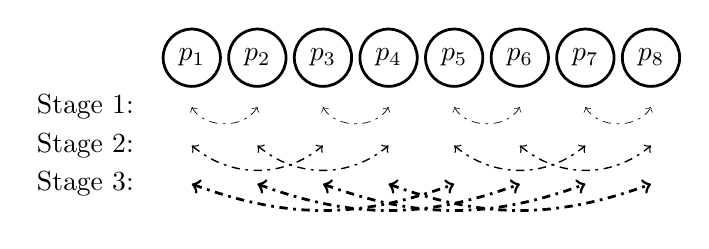
\begin{tikzpicture}[node distance=0.07cm, line width=1pt]
	\tikzstyle{process} = [draw, circle, minimum width = 0.3cm, minimum height = 0.3cm];
	
	\node[process] (p10) {$p_1$};
	\node[process, right = of p10] (p20) {$p_2$};
	\node[process, right = of p20] (p30) {$p_3$};
	\node[process, right = of p30] (p40) {$p_4$};
	\node[process, right = of p40] (p50) {$p_5$};
	\node[process, right = of p50] (p60) {$p_6$};
	\node[process, right = of p60] (p70) {$p_7$};
	\node[process, right = of p70] (p80) {$p_8$};
	
	\def \n {8}
	
	\def \delta {0.0 cm}
	%\def \delta {-0.125 cm}
	\foreach \s in {1,...,\n}
	{
		\node[below = \delta of p\s0] (p\s1) {\phantom{$p_\s$}};
	}
	
	\def \ldelt {0.3cm}
	\node[left = \ldelt of p11] (S1) {Stage 1:};
	
	\def \delta {0.0 cm}
	\foreach \s in {1,...,\n}
	{
		\node[below = \delta of p\s1] (p\s2) {\phantom{$p_\s$}};
	}
	
	\node[left = \ldelt of p12] (S2) {Stage 2:};
	
	\def \delta {0.0 cm}
	\foreach \s in {1,...,\n}
	{
		\node[below = \delta of p\s2] (p\s3) {\phantom{$p_\s$}};
	}
	
	\node[left = \ldelt of p13] (S3) {Stage 3:};
	
	\draw[<->,dash dot, line width=0.25pt] (p11.center) to [out=300,in=240] (p21.center);
	\draw[<->,dash dot, line width=0.25pt] (p31.center) to [out=300,in=240] (p41.center);
	\draw[<->,dash dot, line width=0.25pt] (p51.center) to [out=300,in=240] (p61.center);
	\draw[<->,dash dot, line width=0.25pt] (p71.center) to [out=300,in=240] (p81.center);
	
	\draw[<->,dash dot, line width=0.5pt] (p12.center) to [out=320,in=220] (p32.center);
	\draw[<->,dash dot, line width=0.5pt] (p22.center) to [out=320,in=220] (p42.center);
	\draw[<->,dash dot, line width=0.5pt] (p52.center) to [out=320,in=220] (p72.center);
	\draw[<->,dash dot, line width=0.5pt] (p62.center) to [out=320,in=220] (p82.center);
	
	\draw[<->,dash dot] (p13.center) to [out=340,in=200] (p53.center);
	\draw[<->,dash dot] (p23.center) to [out=340,in=200] (p63.center);
	\draw[<->,dash dot] (p33.center) to [out=340,in=200] (p73.center);
	\draw[<->,dash dot] (p43.center) to [out=340,in=200] (p83.center);
	
	\end{tikzpicture}
	\caption{Static Sparse allreduce: Recursive doubling - Increasing amount of sparse data in every stage}
	\label{fig:ssar_rec_dbl}
\end{figure}

The resulting latency for the \ssarone{} algorithm will be
$L_1(P) = \log_2(P)\alpha,$ as there are $\log_2(P)$ stages. This is
optimal and data-independent.  The runtime will lie in the range
$$L_1(P) + \log_2(P)k\beta_s \leq T_{ssar\_rec\_dbl} \leq L_1(P) +
(P-1)k\beta_s.$$
The lower bound is reached when the $k$ indices fully
overlap.  Therefore, at every stage, $k$ items need to be transmitted as
the intermediate results maintain constant size.  The upper bound is
given when the indices do not overlap at all.  Therefore, at stage $t$,
the number of items transmitted is $2^{t-1}k$. Taking the sum, we get
$$\sum_{i=1}^{\log_2(P)}2^{t-1}k = k\frac{2^{\log_2(P)} - 1}{2-1} =
k(P-1).$$

\subsubsection{The Bandwidth Dominated Case} 

When the data is large, standard dense allreduce implementations make use of Rabenseifner's algorithm~\cite{rabenseifner2004optimization}, which has two steps. 
The first is a ReduceScatter step, which partitions the result vector across nodes, assigning a partition to each node. 
This is implemented by a \emph{recursive halving} technique~\cite{rabenseifner2004optimization}. 
In the second step, the reduced answers are gathered to all other nodes by calling a recursive doubling algorithm as described above. 
This two step algorithm has a total runtime of $$T_{ar\_rab} = 2\log_2(P)\alpha + 2\frac{(P-1)}{P}k\beta_s,$$ which reaches the lower bound on the bandwidth term and is off by a factor $2$ on the latency term. 


We will use a similar blueprint for Sparse allreduce, with some key differences. 
We split the algorithm into two steps: a \emph{Split} phase and a \emph{sparse allgather} phase. 
In the Split phase, we uniformly split the space dimension $N$ into $P$ partitions and assign to each node the indices contained in the corresponding partition. 
We split each sparse vector at its node and directly send each subrange of indices to the corresponding recipient in a \emph{sparse} format. 
This direct communication comes at a theoretical price of higher latency cost, but by using non-blocking send and receive calls, the computation and communication can be nicely overlapped.
%Figure~\ref{fig:direct_sparse_alltoall} depicts this communication pattern. 
Each node then reduces the data it received and builds the result for its partition. 
In the second phase, the data has to be gathered to all other nodes by using the previously described sparse allgather.
%This sparse allgather is executed by a recursive doubling algorithm with efficient sparse summation as described in the previous section.

%\begin{figure}[htbp]
%	\begin{center}
%		\begin{tikzpicture}[node distance=0.2cm, line width=1pt]
%		\tikzstyle{process} = [draw, circle, minimum width = 0.5cm, minimum height = 0.5cm];
%		
%		\def \n {8}
%		
%		\node[process] (p10) {$p_1$};
%		\node[process, right = of p10] (p20) {$p_2$};
%		\node[process, right = of p20] (p30) {$p_3$};
%		\node[process, right = of p30] (p40) {$p_4$};
%		\node[process, right = of p40] (p50) {$p_5$};
%		\node[process, right = of p50] (p60) {$p_6$};
%		\node[process, right = of p60] (p70) {$p_7$};
%		\node[process, right = of p70] (p80) {$p_8$};
%		
%		\def \delta {1.0 cm}
%		\foreach \s in {1,...,\n}
%		{
%			\node[process, below = \delta of p\s0] (p\s1) {$p_\s$};
%		}
%		
%		\foreach \k in {1,...,\n}
%		{
%			\foreach \s in {1,...,\n}
%			{
%				\ifnum\k=\s
%				%nothign
%				\else
%				\draw[->, dotted, shorten >=4pt, line width=0.25pt] (p\k0.south) to (p\s1.north);
%				\fi
%			}
%		}
%		
%		\end{tikzpicture}
%		\caption{Direct Sparse Send Alltoall}
%		\label{fig:direct_sparse_alltoall}
%	\end{center}
%\end{figure}

\noindent Obtaining runtime bounds for \ssartwo{} is slightly more involved. The Split part takes time $$(P-1)\alpha + 0\beta_s \leq T_{split} \leq (P-1)\alpha + k\beta_s.$$ 
Notice that both extremes imply that each node has $k$ items for the sparse allgather and thus $\mathcal{K} = k \times P$ is reached. For this second step in the algorithm to be optimal, every node must have an intermediate result of size $\frac{k}{P}$, as we want the final result to have a size $\mathcal{K} = k$ and the communication to be equally distributed. 

For every node to have an intermediate result of the desired size, we know that each node has to send at least $\frac{P-1}{P}k$ items to other nodes. Otherwise, if every node has exactly $k$ items, we reach the upper bound for the result size of $\mathcal{K} = k \times P$. So we get $$L_1(P) + \frac{P-1}{P}k\beta_s \leq T_{sparse\_ag} \leq L_1(P) + (P-1)k\beta_s.$$
The algorithm latency is again data-independent: $$L_2(P) = (P-1)\alpha + L_1(P).$$
Combining these terms yields 
$$L_2(P) + 2\frac{P-1}{P}k\beta_s \leq T_{ssar\_split\_ag} \leq L_2(P) + Pk\beta_s.$$

\subsubsection{The Dynamic Case: Switching to Dense} 

The discussion so far focused on the case where maintaining a sparse representation is efficient. 
However, as we gather data, the size of the result $\mathcal{K}$ might become larger than the sparsity-efficient threshold $\delta$, in which case we switch to a dense representation. 
This is the \emph{dynamic} version of the problem (DSAR).
In this case, the following lower bound on the efficiency of the algorithm will hold.

\begin{theorem}
	Any algorithm solving the DSAR problem needs at least time $\log_2(P)\alpha + N\beta_d$.
	\label{lem:dsar_min_dur}
\end{theorem}

The proof follows directly on the latency term and directly holds on the bandwidth term from the fact, that each node has to receive or send at least $N-k$ items in order to become dense. From this observation we derive the following lemma, which says that, in this dynamic case, one can only hope to get a speedup of at most factor $2$ compared to an optimal \emph{dense} allreduce algorithm,  focusing on the bandwidth term.

\begin{lemma}
	The bandwidth required by any algorithm for the DSAR problem is at least $\frac{1}{2}$ that of a bandwidth-optimal dense allreduce algorithm.
\end{lemma}
\begin{proof}
	Notice that the dense allreduce with $k=N$ has a lower bound of $2\frac{P-1}{P}N\beta_d$ on the bandwidth if computation is equally distributed. From Theorem \ref{lem:dsar_min_dur} we know that every DSAR algorithm has a minimum bandwidth term of $N\beta_d$, which is obviously bigger than $\frac{P-1}{P}N\beta_d$ for any $P$.
\end{proof}

Based on these insights, our solution for DSAR adapts the previous two-stage algorithm to exploit the fact that every reduced split will become dense. \dsar{} hence receives the data in a sparse format from all the other nodes in the first phase, then switches the representation and performs a dense allgather in the second stage. Here, we can leverage existing implementations, which are highly optimized to perform this second step with dense data. Based on the known times needed by those algorithms, which are obviously input density independent, we derive the running time for our algorithm given both extremes. The latency is again $L_2(P)$. Combined, we get $$L_2(P) + \frac{P-1}{P}N\beta_d \leq T_{dsar\_split\_ag}$$and $$T_{dsar\_split\_ag} \leq L_2(P) + k\beta_s + \frac{P-1}{P}N\beta_d.$$

\paragraph{Stochastic Analysis.} In the additional material, we present an analysis of our algorithm in a stochastic setting, where the $k$ non-zero indices at each processor are chosen randomly.

\section{Artifact and Additional Features}
\label{sec:additional-features}

\paragraph{Interface and Code.} The \mml{} library provides an interface
that is similar to that of standard MPI calls, with the
caveat that the data representation is assumed to be a sparse stream.
Given this, the changes needed to port MPI-enabled code to exploit
sparsity through \mml{} are minor.  The library implementation consists
of around 2,000 lines of native \verb!C++11!. (This does not include
infrastructure such as benchmarks and tests which would raise the line
count by an order of magnitude.) Adding \mml{} to CNTK required changing
around $100$ lines of code. 
%While efficient sparse-input collectives are the key component of \mml{}, it
%has some additional non-trivial features. In particular, we implement
%\emph{non-blocking} versions of these protocols, and support
%\emph{low-precision data representation}.

\paragraph{Non-Blocking Operations.}
%Due to the large computational and communication cost of machine learning algorithms, it is often beneficial to be able to overlap communication and computation.
We also implement the previous algorithms in a \emph{non-blocking way}.
Specifically, we allow a thread to trigger a collective operation, such
as allreduce, in a nonblocking way. This enables the thread to proceed
with local computations while the operation is performed in the
background. 
%
For deep networks, we can nicely overlap communication and computation
during the gradient aggregation phase by calling the aggregation per
layer in a non-blocking fashion.  As of MPI-3, implementations support
non-blocking collective operations.  However, rendering a custom
operation implementation non-blocking is not entirely
straightforward~\cite{libnbc, hoefler-sc07} and needs to consider subtle
message progression issues~\cite{hoefler-ib-threads}. 
%
%
%
%We implement the \ssarone{} algorithm in a non-blocking fashion based on LibNBC~\cite{libnbc}, which provides a non-blocking interface for MPI collective operations~\cite{hoefler2006design}. Since the \dsar{} algorithm relies on a allgather in the second phase, we are able to implement the algorithm in a non-blocking fashion by utilizing direct non-blocking send and receive calls in the first phase of the algorithm, and then making use of the MPI library specific non-blocking allgather implementations.

\begin{figure*}[htbp]
	\centering
	%	\subcaptionbox{Piz Daint}[0.355\textwidth]{
	\includegraphics[width=0.345\textwidth,height=\textheight,keepaspectratio]{pipeline_daint}
	%	}
	%	\subcaptionbox{Greina (GigE)}[0.545\textwidth]{
	\includegraphics[width=0.555\textwidth,height=\textheight,keepaspectratio]{pipeline_greina}
	%	}
	\caption{Data density versus reduction time for various algorithms, dimension $N=16\textrm{M}$ and $P=8$ nodes.}
	\label{fig:ComparePipeline}
\end{figure*}

\paragraph{Low-Precision Support.}
To further reduce bandwidth cost, \mml{} supports lower-precision data
representation for the updates, using QSGD
quantization~\cite{alistarh2016qsgd}, which provably preserves the
correctness of the algorithm. In brief, in this variant, each vector is
split into \emph{buckets} of size $B$ (in the order of 1,024) and each
bucket is quantized independently and  stochastically. Thus, each bucket
corresponds to $B$ \emph{low-precision data items}, e.g., 4-bit integers,
packed to reduce space and a full-precision \emph{scaling factor}.  We
focus on low-precision to reduce the bandwidth cost of the \emph{dense}
case. Hence, in the low-precision implementation, we either omit
sparsity, or we use the low-precision data representation for the second
part of the \dsar{} algorithm, where the data becomes dense.
%Adding low-precision support to \dsar{} is not trivial; however, due to space
%constraints, we leave the system description to the full version of our
%paper.
Interestingly, by making use of this functionality, we are able
to achieve speedup higher than  $2\times$ compared to a fully dense
allreduce, which was the upper bound when working with full-precision
data. 
%
%
%: more precisely, we now  split the universe size $N$ uniformly into $P$ parts, where every node does the computation on its part of the vector. The data is quantized and sent directly to the corresponding recipient. After having aggregated all the received data, every node will directly redistribute the newly quantized results to all other nodes. For mixing sparsity awareness and low-precision support, we implement the first phase of the \dsar{} algorithm with direct send of the sparse streams on parts of the entire vector as previously described. Then, as the data is forced to be stored in a dense format at every node, it can be quantized after having received all the data from the other nodes. By making use of this functionality, we are able to achieve an overall speedup higher than  $2\times$ compared to a fully dense allreduce, which we showed to be an upper bound when working with full-precision data. 

\section{Experiments}

%\begin{figure*}[htbp]
%	\centering
%	\subcaptionbox{Piz Daint}[0.45\textwidth]{
%		\includegraphics[width=0.4\textwidth,height=\textheight,keepaspectratio]{img/output_daint}
%	}
%	\subcaptionbox{Greina (GigE)}[0.45\textwidth]{
%		\includegraphics[width=0.4\textwidth,height=\textheight,keepaspectratio]{img/output_greina}
%	}
%	\caption{Data density versus reduction time for various algorithms, dimension $N=16\textrm{M}$ and $P=8$ nodes.}
%	\label{fig:CompareSystem}
%\end{figure*}

\paragraph{Setup.} 
We now validate \mml{} on real world applications and synthetic
experiments.
%Complete code and experimental logs will be made available once the paper is de-anonymized.
Our experiments target two important scenarios:
supercomputing and cloud computing.  For the first setting, we execute
on the CSCS Piz Daint supercomputer~\cite{PizDaint}, with Cray XC50
nodes, each of which has a 12 cores HT-enabled Intel Xeon E5-2690 v3 CPU
with 4GB RAM and an NVIDIA Tesla P100 16GB GPU. Piz Daint is currently
the most powerful supercomputer in Europe (3rd in the world) and has a
high-performance Cray Aries interconnect with a Dragonfly network topology.
For the second setting, we use Amazon EC2 instances with a similar CPU
configuration, but relatively older NVIDIA K80 GPUs, connected
through Gigabit Ethernet.  We perform additional tests on a
cluster called Greina, with CX50 nodes and an InfiniBand FDR or 
Gigabit Ethernet interconnect and on a production-grade GPU cluster, described in the corresponding section.  

%We measure the MPI point-to-point bandwidth of each system with standard
%ping-pong techniques. Piz Daint reaches a bandwidth of up to 50
%Gbps, Greina achieves roughly 1 Gbps using the Gigabit Ethernet
%(GigE) interconnect, and around 40 Gbps when using the InfiniBand FDR (IB)
%interconnection. The Amazon cluster bandwidth saturates at 4 Gbps.

In all our experiments, the baseline will be the MPI allreduce implementation on the fully dense vectors. 
On EC2, we make use of the default Open MPI installation optimized by Amazon. 
On Piz Daint, we compare against the custom Cray-MPICH installation, highly optimized by Cray. Since our problems usually have dimension $N > 65 \textrm{K}$,  
we fix the datatype for storing an index to an \verb!unsigned int!.

\begin{table}[b]
	\centering
	\begin{tabular}{ @{} l | r | r | r @{} }
		\toprule
		Name & \# Classes & \# of samples & Dimension \\
		\midrule 
		URL~\cite{ma2009identifying} & 2 & 2 396 130 & 3 231 961 \\
		Webspam~\cite{webb2006introducing} & 2 &  350 000 & 16 609 143 \\
		\midrule 
		ImageNet~\cite{russakovsky2015imagenet} & 1000 & 1,2 million & 256x256x3\\
		MNIST~\cite{lecun2010mnisthandwrittendigit} & 10 & 60 000 & 28x28 \\
		CIFAR-10~\cite{krizhevsky2009learning} & 10 & 60 000 & 32x32x3 \\
		\midrule
		ATIS~\cite{hemphill1990atis} & 128 & 4 978 \textit{s} / 56 590 \textit{w} & - \\
		\midrule
		Hansards~\cite{hansards} & - & 948K \textit{s} / 15 657K \textit{w} & - \\
		\bottomrule
	\end{tabular}
	\caption{Real World Application Datasets. \textit{s} stands for sentences (or pairs) and \textit{w} for words. }
	\label{tbl:DataSets}
\end{table}

\subsection{Micro-Benchmarks and Large-Scale Regression}

We begin by validating our theoretical analysis on synthetic data, on the Piz Daint and Greina (GigE) clusters. 
We vary the data dimension $N$ and the data density $d$ as well as the number of nodes $P$. 
Based on the defined density, $k$ indices out of $N$ are selected uniformly at random at each node and are assigned a random value. 
We run our sparse allreduce algorithms in order to validate both correctness and the relative ordering of the derived analytical bounds. 
The choice of parameters to generate the data, is within reasonable ranges, seen in real world datasets. 
(E.g., we pick data dimensions corresponding to common layer sizes in neural networks.) 

For readability, graphs are in a log-log scale. 
As execution times are non-deterministic, we conduct five experiments with newly generated data, while running each one for ten times. 
Based on those 50 resulting runtime values, we state the 25 and 75 percentage quantiles.

Following the theoretical analysis, we expect the variant \ssarone{} to perform best for a small amount of data, when latency dominates over the bandwidth term. At higher node count $P$, data becomes larger, which leads to less improvement of the algorithm \ssarone{} at the same number of non-zero entries over the other variants. 
Furthermore, the algorithm  \ssartwo{} dominates over the \dsar{} variant as long as the number of non-zero indices is relatively low compared to the overall reduced size. 
To show the impact of the network on performance, we run identical tests on both Piz Daint and Greina (GigE) in Figure~\ref{fig:ComparePipeline}.
The results confirm our analysis. 

Additionally, the experiments in Figure~\ref{fig:ComparePipeline} also compare our approaches against a ring-based MPI dense allreduce and its sparse counterpart. We note that, on a fast network and relatively small number of nodes, the ring-based algorithm is faster by a slight margin on the dense case, whereas the sparsity-based approach is more competitive on a relatively slower Gigabit Ethernet connection. 

%\begin{figure*}[htbp]
%	\centering
%	\subcaptionbox{Training error}[0.45\textwidth]{
%		\includegraphics[width=0.4\textwidth,height=\textheight,keepaspectratio]{img/mnist_train}
%	}
%	\subcaptionbox{Test accuracy}[0.45\textwidth]{
%		\includegraphics[width=0.4\textwidth,height=\textheight,keepaspectratio]{img/mnist_test}
%	}
%	\caption{MNIST convergence for various algorithm variants.}
%	\label{fig:MnistConvergence}
%\end{figure*}


%\begin{figure}[htbp]
%	\centering
%	\subcaptionbox{$N=4\textrm{M}$ / $P=32$}[0.45\textwidth]{
%		\includegraphics[width=0.4\textwidth,height=\textheight,keepaspectratio]{img/synthetic1}
%	}
%%	\subcaptionbox{$N=4\textrm{M}$ / $P=128$}[0.45\textwidth]{
%%		\includegraphics[width=0.4\textwidth,height=\textheight,keepaspectratio]{img/synthetic1}
%%	}
%	\caption{Synthetic Data Micro-Benchmarks on Piz Daint.}
%	\label{fig:SyntheticData}
%\end{figure}


\paragraph{Large-Scale Regression.}
We use MPI-OPT to train linear classifiers (Logistic Regression, SVM) on large-scale classification datasets using SGD and SCD.
The goal is to examine the runtime improvements by just exploiting the sparsity inherently present in the datasets and algorithms.
The datasets are specified in Table~\ref{tbl:DataSets}. We make use of the binary classification datasets URL and Webspam.

%\begin{table*}[htbp]
%	\begin{footnotesize}
%	\centering
%	\begin{tabular}{ @{} l | l | l | r | r | l | r | r @{} }
%		\toprule
%		System & Dataset & Model & \# of nodes & Baseline Time (m) & Algorithm & Algo. Time (m) & Speedup \\
%		\midrule
%		\multirow{ 1}{*}{Piz Daint} & \multirow{ 1}{*}{ImageNet} & \multirow{ 1}{*}{VGG19} & \multirow{ 1}{*}{8} & \multirow{ 1}{*}{61.23 (32.72)} & Q4 & 39.49 (9.87) & \textbf{1.55 (3.31)} \\
%%		Piz Daint & ImageNet & VGG19 & 8 & 61.23 (32.72) & Q4 & 39.49 (9.87) & \textbf{1.55 (3.31)} \\
%%		\midrule
%%		Piz Daint & ImageNet & AlexNet & 16 & 33.69 (26.82) & Q4 & 25.83 (19.77) & \textbf{1.30 (1.36)} \\
%%		\midrule
%%		Piz Daint & \multirow{ 2}{*}{CIFAR-10} & \multirow{ 2}{*}{ResNet110} & \multirow{ 2}{*}{8} & 0.70 (0.23) & Top16\_Q4 & 0.82 (0.35) & 0.85 (0.66) \\
%%		EC2 & & & & 0.97 (0.34) & Top16\_Q4 & 0.90 (0.24) & \textbf{1.08 (1.40)} \\
%%>>>>>>> 15e2b074016d25b678ae2360cb3f29878a13c18b
%		\midrule
%		\multirow{ 1}{*}{Piz Daint} & \multirow{ 1}{*}{ImageNet} & \multirow{ 1}{*}{AlexNet} & \multirow{ 1}{*}{16} & \multirow{ 1}{*}{33.69 (26.82)} & Q4 & 25.83 (19.77) & \textbf{1.30 (1.36)} \\				\midrule
%		Piz Daint & \multirow{ 2}{*}{MNIST} & \multirow{ 2}{*}{MLP} & \multirow{ 2}{*}{8} & 1.78 (1.65) & Top16\_Q4 & 0.49 (0.36) & \textbf{3.65 (4.53)} \\
%		EC2 & & & & 24.41 (24.18) & Top16\_Q4 & 1.28 (1.05) & \textbf{19.12 (22.97)} \\
%		\bottomrule
%	\end{tabular}
%  \caption{Training neural networks using CNTK. The times represent average time in minutes for a full dataset pass, and its communication part in brackets. Speedup versus dense MPI is shown end-to-end, with communication speedup in brackets.}
%	\label{tbl:ResutlsCntkVision}
%	\end{footnotesize}
%\end{table*}

For SGD, the
samples (and hence, gradients) have high sparsity since the features are
trigrams: while many such combinations exist, an item, e.g., a sentence,
can only have a very limited set of them present. This is extremely
common in text-based datasets. Since communication is lossless,
convergence is preserved and we only report speedup of the communication
and overall training time. We run SGD with large batches (1,000 $\times
P$) for various combinations.  The achieved speed of MPI-OPT with the
best sparse reduction algorithm is reported in
Table~\ref{tbl:ResutlsMpiOpt}. 

\begin{table*}[htbp]
	\begin{footnotesize}
		\centering
		\begin{tabular}{ @{} l | l | l | r | r | l | r | r @{} }
			\toprule
			System & Dataset & Model & \# of nodes & Baseline Time (s) & Algorithm & Algo. Time (s) & Speedup \\
			\midrule
			\multirow{ 3}{*}{Piz Daint} & \multirow{ 3}{*}{Webspam} & LR & 32 & 2.40 (2.16) & \multirow{ 3}{*}{\ssarone} & 0.68 (0.35) & \textbf{3.53 (6.17)} \\
			%			&  & LR & 128 & 0.64 (0.58) & & 0.18 (0.10) & \textbf{3.56 (5.80)} \\
			&  & SVM & 32 & 1.62 (1.42) & & 0.65 (0.44) & \textbf{2.49 (3.23)} \\
			\midrule
			\multirow{ 3}{*}{Piz Daint}& \multirow{ 3}{*}{URL} & LR & 32 & 2.64 (2.58) & \multirow{ 3}{*}{\ssarone} & 0.75 (0.70) & \textbf{3.52 (3.69)} \\
			%			&  & LR & 128 & 0.57 (0.56) &  & 0.29 (0.28) & \textbf{1.97 (2.00)} \\
			&  & SVM & 32 & 1.98 (1.93) &  & 0.56 (0.53) & \textbf{3.54 (3.64)} \\
			\midrule
			\multirow{ 2}{*}{Piz Daint}& Webspam & LR & 8 & 4.67 (3.79) & \multirow{ 2}{*}{\ssartwo} & 2.56 (1.58) & \textbf{1.82 (2.40)} \\
			& URL & LR & 8 & 3.77 (3.53) & & 2.09 (1.50) & \textbf{ 1.80 (2.35)} \\
			\midrule
			\multirow{ 2}{*}{Greina (IB)} & Webspam & LR & 8 & 6.52 (4.67) & \multirow{ 2}{*}{\ssartwo} & 3.63 (1.90) & \textbf{1.80 (2.46)} \\
			& URL & LR & 8 & 8.14 (4.47) & & 6.11 (2.49) & \textbf{1.33 (1.80)} \\
			\midrule
			\multirow{ 2}{*}{Greina (GigE)} & Webspam & LR & 8 & 76.80 (75.95) & \multirow{ 2}{*}{\ssartwo} & 3.79 (2.95) & \textbf{20.26 (25.75)} \\
			& URL & LR & 8 & 104.50 (100.46) & & 8.26 (4.22) & \textbf{12.65 (23.81)} \\
			\bottomrule
		\end{tabular}
		\caption{Distributed optimization using MPI-OPT. The times are averages for a full dataset pass, with the communication part in brackets. Speedup versus dense MPI is shown end-to-end, with communication speedup in brackets.}
		\label{tbl:ResutlsMpiOpt}
	\end{footnotesize}
\end{table*}

Additionally, we run SCD incorporated in
MPI-OPT following the distributed implementation
of~\cite{liu2015asynchronous}. We run the optimization on the logistic
regression loss function for the URL dataset distributed on 8 nodes of
Piz Daint to achieve identical convergence compared to SGD. Every node
contributes 100 indices after every iteration. As the values calculated
by each node lie in different slices of the entire model vector, we
compare the runtime of an sparse allgather from \mml{} to its dense
counterpart. MPI-OPT with a dense allgather has an average epoch time of 49 seconds, with 24 seconds dedicated to communication. The sparse allgather executes a dataset pass (epoch) in 26 seconds on average, with 4.5 seconds spent in the communication layer. This implies an overall speedup of factor $\bm{1.8}\times$, due to a $\bm{5.3}\times$ speedup in communication time.


\paragraph{Comparison with Apache Spark.} Next, we compare MPI-OPT with Apache Spark v1.6, which is officially supported by CSCS~\cite{CSCSSpark}.  Comparison is performed on the same datasets, with the note that Spark uses its own communication layer and does not exploit sparsity. 
On the Piz Daint supercomputer, using $8$ nodes, MPI-OPT with \mml{} reduces the time to convergence on the URL dataset by $\bm{63\times}$.
This is largely due to the reduction in communication time, which we measure to be of $\bm{185\times}$. Concretely, the average epoch time is reduced from 378 seconds, with 319 seconds spent for communication, to an average of 6 seconds per epoch, whereof 1.7 seconds represent the communication time.
Compared to Spark, MPI-OPT with the standard Cray-optimized \emph{dense} allreduce has a $31\times$ speedup to convergence, due to a $43\times$ speedup in communication time. An epoch is executed in 13 seconds on average, with 8.6 seconds spent on communication. We further investigated these speedups on an 8-node research cluster
with a Gigabit Ethernet interconnection. This mimics an Amazon EC2 scenario, with no background traffic. Using MPI-OPT, the average
training time per epoch drops from 1,274 seconds (Spark) to 14 seconds,
representing a speedup of $\bm{86\times}$. On the communication part,
the time per epoch drops from 1,042 seconds to 6 seconds. The communication time and
overall speedup of a \emph{dense} allreduce over Spark's communication layer are both of factor {$\bm{12\times}$}.

\subsection{Training Deep Neural Networks}

Next, we turn to training state-of-the-art deep neural networks in CNTK, using \mml{}.  
To exploit sparsity, we use the Top-$k$ SGD algorithm~\cite{dryden2016communication, sun2017meprop, aji2017sparse}, combined with low-precision support~\cite{alistarh2016qsgd}. 
We execute three types of tasks: \emph{image classification} on the
ImageNet, CIFAR-10, and MNIST datasets, \emph{natural language
	understanding} on the ATIS corpus and \emph{machine translation} on the
Hansards dataset. The datasets are specified in
Table~\ref{tbl:DataSets}. For vision, we run experiments on the
following deep networks: AlexNet~\cite{AlexNet},
VGG~\cite{simonyan2014very}, ResNet~\cite{he2016deep} and multi layer
perceptrons (MLPs) with fixed numbers, two hidden layers of dimension 4,096 each. For natural language understanding and machine translation we use an encoder-decoder network consisting of two LSTM~\cite{hochreiter1997long} cells each. 

For this, we have interfaced \mml{} into CNTK. We make use of the
non-blocking version of the sparse allreduce algorithm when working with
full precision. Selecting the biggest elements in magnitude is
implemented efficiently in CNTK by building ``buckets" with 512
consecutive tensor elements each (reshaping the tensor when necessary),
and implementing a fast randomized Top-$k$ algorithm. This enables fast
computation on GPUs and allows for significant speedup over the fully
dense allreduce variant.
%We omit selecting the Top-$k$ values and
%quantization of gradient matrices with small ($<10K$) size, as the computational effort of either operation exceeds the overall reduction in time given by reducing the amount of data transmitted.
We use standard batch sizes and default hyper-parameters for 32-bit full accuracy convergence in all our experiments. These values are given in the open-source CNTK 2.0 repository. We have also experimented with supporting the 1-bit SGD quantization algorithm~\cite{seide20141} and asynchronous (ASGD) training. Unfortunately, for 1-bit SGD, the way tensors in convolutional layers are handled, can actually \emph{increase} overall training time with respect to the MPI baseline in networks with lots of convolutions, such as ResNet. ASGD training requires extremely careful hyperparameter tuning to maintain accuracy~\cite{zhang2017yellowfin} and is therefore left for future work.


\paragraph{Accuracy \& Speedup. } As stated by in the preliminaries, working with delayed consistency might affect convergence speed, as the sparsity-accuracy trade-offs are not yet fully understood. Similarly to~\cite{dryden2016communication, aji2017sparse}, experiments on MNIST with multi-layer perceptrons (MLPs), CIFAR-10 on ResNet110 and ATIS with LSTMs show almost identical convergence speed even when forcing high sparsity. When combining Top-$k$ and quantization with selecting $k=16$ out of every bucket of size 512 and quantizing the dense values using 4-bit precision we achieve a top-1 accuracy $0.48\%$ below the full precision and even increase top-5 accuracy by $0.12\%$ on the CIFAR-10 dataset. For MNIST, the training error fluctuates by less than $0.1\%$. Comparing the overall epoch time on this last task to a full dense reduction implementation reveals its impact of system choice. We achieve a overall speedup of factor $\bm{19.12\times}$ on a 8 node Amazon EC2 cluster with Gigabit Ethernet interconnection, whereas the speedup factor on the high performance network on Piz Daint reaches a factor $\bm{3.65\times}$. We furthermore conduct neural machine translation experiments on the Hansards dataset using an encoder-decoder network with two LSTM cells each. By selecting the  4 largest values out of each 512 consecutive elements, we achieve an overall speedup of factor $\bm{1.54\times}$ with slightly worse convergence speed on 8 nodes of Piz Daint.
%The impact of different $k$ values for this dataset is visible in Figure~\ref{fig:MnistConvergence}.

We have also applied Top-$k$ SGD on the ImageNet dataset, but found that reaching full accuracy requires significant additional hyper-parameter tuning. 
Recent work reports accurate training at extremely high sparsity levels on this dataset~\cite{lin2017deep}, but we were not able to successfully replicate these results on our setup within our computational budget. 
%For this reason, we only employ low precision (quantization to 4bits) in \mml{} when executing our benchmarks on the ImageNet dataset, in which case we achieve convergence.  

%\paragraph{Speedup.}  In Table~\ref{tbl:ResutlsCntkVision}, we provide the overall epoch time, and the time spent communicating for various image classification models and training algorithms. \emph{Q4} denotes the 4-bit quantized version on all the gradient values. \emph{Top16} represents the version where the biggest 16 values in magnitude are selected per buckets of 512 consecutive tensor values. We give the speedup for those values of $k$ in combination with 4-bit low precision on the dense values in the second part of the algorithm based on the previous convergence tests. . 

%Further, we conduct neural machine translation experiments on the Hansards dataset using an encoder-decoder network with two LSTM cells each. By selecting the  4 largest values out of each 512 consecutive elements, we achieve an overall speedup of factor $\bm{1.54\times}$ with slightly worse convergence speed on 8 nodes of Piz Daint. For natural language understanding problems on the ATIS dataset, using an identical network, we obtain a overall speedup of $\bm{2.6\times}$ to full convergence, compared to a full dense allreduce, by only selecting the biggest 2 values out of buckets of 512 elements.

\begin{figure*}[htbp]
	\centering
	\subcaptionbox{Numbers are for $6$ training passes over the entire dataset, recording training error (CE loss). Validation results (word-error-rates) are discussed in the text.\label{fig:production-accuracy-vs-time}}[0.45\textwidth]{
		\includegraphics[width=0.4\textwidth,height=\textheight,keepaspectratio]{ms_experiment_convergence}
	}
	\subcaptionbox{SparCML Scalability\label{fig:production-scalability}}[0.355\textwidth]{
		\includegraphics[width=0.305\textwidth,height=\textheight,keepaspectratio]{ms_experiment_scalability}
	}
	\caption{Production Workload Speech Experiments.}
	\label{fig:ProductionWorkload}
\end{figure*}

\subsection{Production Workload Experiments}

The final test of our framework is on a state-of-the-art acoustic model for automated speech recognition (ASR), powering a popular digital personal assistant. 
%Due to anonymization constraints, some details of our setup are omitted. 
The model we train is a state-of-the-art LSTM network with attention. The model has more than 60 million parameters, 2.4 million of which reside in the attention layer. 
We employ Top-$k$ SGD for the training of the attention layer, starting from a pre-trained LSTM network. 
The dataset consists of approximately 30,000 hours (3.5 years) of annotated speech. 
Our cluster deployment consists of 32 server nodes, each with four NVIDIA V100 GPUs, totalling 128 GPUs. 
Aggregation inside each node is performed via NVIDIA NCCL~\cite{NCCL}. 

The baseline we compare against is training on 4 nodes, 16 GPUs in total, without sparsity or quantization, but employing a carefully-tuned instance of block-momentum SGD (BMUF)~\cite{Block-Momentum-SGD}. 
Higher node counts for this variant lead to negative scalability and, in some cases, divergence. 
We note that this baseline already performs non-trivial communication reduction, since it communicates updates less frequently between nodes with respect to standard minibatch SGD.
(Standard minibatch SGD is infeasible on our setup due to the large model size and node count.)

We execute the standard training protocol for this model: six training passes over the entire dataset, registering the time to complete the experiment and the training accuracy, after which we perform validation on a series of proprietary datasets which have not been used during training. In this second stage, we record word-error-rates (WER) for the model. 
The 16 GPU BMUF baseline takes approximately 14 days to complete training. 
We compare against our version of Top-$k$ SGD with~\mml{}, in which gradients are split into groups of 512 consecutive coordinates, out of which we select the 4 largest ones, which we transmit from each group, saving the rest locally. 
This corresponds to $<0.8\%$ density of the gradient updates. We aim to leverage the fact that, in this production setting, most updates will occur in the parameters of the attention layer. 

Figure~\ref{fig:production-accuracy-vs-time} presents the results in training-error-versus-time format, where error is measured by standard cross-entropy (CE) loss, using our implementation, for 32, 64, and 128 GPUs. 
We highlight the fact that the sparse implementation is able to reach similar accuracy in a fraction of the time: at 128 GPUs, we are able to reduce training time to $<1.8$ days.  
Figure~\ref{fig:production-scalability} highlights the good scalability of the method. 
We closely examined the test error in terms of word-error-rate (WER) for the converged models, on validation sets. 
We found that the models trained with SparCML incur error rates that usually \emph{on par} with the full-precision baseline: errors are less than $1\%$ higher than full-precision (but unscalable) training and sparse training can \emph{improve} accuracy by up to $1\%$ on some validation datasets.   
This trade-off is very advantageous for our application scenario. 

\section{Related Work}

There has been a surge of interest in distributed machine learning; see Ben-Nun and Hoefler~\cite{distdl-preprint} for a survey. We will focus on references that are closely related to our work. 

\paragraph{Reduced Communication Techniques.} 
Seide et al.~\cite{seide20141} was among the first to propose quantization to reduce the bandwidth and latency costs of training deep networks. 
More recently, Alistarh et al.~\cite{alistarh2016qsgd} introduced a theoretically-justified distributed SGD variant called Quantized SGD (QSGD), which allows the user to trade off compression and convergence rate. 
We implement QSGD as a default quantization method.  

Dryden et al.~\cite{dryden2016communication} and Aji and Heafield~\cite{aji2017sparse} considered an alternative approach to communication reduction for data-parallel SGD, \emph{sparsifying} the gradient updates by only applying the top-$k$ components, taken at at every node, in every iteration, for $k$ corresponding to $<1\%$ of the update size. Since then, other references~\cite{sun2017meprop, lin2017deep} explored this space, showing that extremely high gradient sparsity ($<0.1\%$) can be supported by convolutional and recurrent networks with preserved accuracy, although maintaining accuracy requires very careful tuning of hyperparameters. 

We complement this work by providing  efficient sparsity support, with consistent runtime gains in large-scale settings. 

\paragraph{Lossless Methods.} One loss-less communication-reduciton technique is \emph{factorization}~\cite{chilimbi2014project, xing2015petuum}, effective in deep neural networks with large fully-connected layers. This is less applicable in networks with large convolutional layers, which is the case for for many modern architectures~\cite{he2016deep, szegedy2017inception}. Poseidon / Petuum~\cite{xing2015petuum} is a complete distributed machine learning framework built on the idea of reducing communication through factorization. 
A second such method is executing \emph{extremely large batches}, thus hiding the cost of communication behind larger computation~\cite{goyal2017accurate, you2017scaling}. 
Although promising, large-batch methods require careful per-instance parameter tuning and do not eliminate communication costs. 

\paragraph{Communication Frameworks.} Several frameworks have been proposed for reducing communication cost of distributed machine learning. 
One popular example is NVIDIA's NCCL framework~\cite{NCCL}, which significantly reduces communication cost when the nodes are NVIDIA GPUs and the proprietary NVLINK interconnect is available, which is not the case in multi-node settings, such as supercomputing. Further, NCCL currently only implements a very restricted set of reduction operations.
In addition, there is a non-trivial number of frameworks customized to specific application scenarios, such as the Livermore Big Artificial Neural Network Toolkit (LBANN)~\cite{van2015lbann} or S-Caffe~\cite{awan2017s}.
While very efficient in specific instances, these frameworks do not usually leverage reduced-communication techniques, or sparsity. 

\paragraph{Sparse Reduction.} Efficient MPI support for reductions over sparse input vectors was considered by~\cite{hofmann2008mpi} and from the algorithmic perspective in~\cite{traff2010transparent}. 
The first reference proposes and evaluates a direct runlength encoding approach; we significantly extend this approach in the current work, including the observation that data might become dense during the reduction process and that an efficient and flexible data representation must be provided in this case. Kylix~\cite{zhao2014kylix} considers sparse many-to-many reductions in the context of computation over large scale distributed graph data on community clusters. However, Kylix assumes knowledge of the data distribution and performs multiple passes over the reduction, which make it not applicable to our scenario. 
Dryden et al.~\cite{dryden2016communication} implement a sparse variant of the classical allreduce algorithm via a pairwise reduce-scatter followed by a ring-based allgather. The amount of data is kept constant at every stage of their algorithm by re-selecting the top $k$ values and postponing the other received values. We note that this ability to preserve a local residual is specific to Top-$k$ SGD and that our framework is more general. In terms of performance, their implementation will provide similar results to our \ssartwo{} implementation. 

%\paragraph{Reduced Communication Techniques.} One of the earliest
%to address the bandwidth and latency costs of
%training large-scale deep neural networks are Seide et
%al.~\cite{seide20141}. 
%%Their work can be placed in the context of a
%%larger push towards communication-avoiding algorithms in large-scale
%%settings distributed settings, e.g.~\cite{DemmelTutorial}.  
%They proposed one-bit SGD, a communication-efficient variant of the
%data-parallel SGD algorithm, which reduces each floating-point
%coordinate to \emph{a single bit (its sign)}, and accumulates the
%resulting error locally. 
%%
%Seide et al. demonstrated convergence empirically~\cite{seide20141}, and
%a variant of it is now available by default in the Microsoft Cognitive
%Toolkit (CNTK)~\cite{CNTK}, although its convergence properties are
%still not well understood. 
%%
%More recently, Alistarh et al.~\cite{alistarh2016qsgd} introduced a
%theoretically-justified distributed SGD variant called Quantized SGD
%(QSGD), which allows the user to trade off the update compression with
%the convergence rate. 
%%
%In brief, they show that communication can be quantized to four bits
%of precision, and still converge to the same target accuracy for a wide
%range of state-of-the-art networks. We exploit this finding in this
%work, and implement QSGD as a default quantization method.  
%
%Recent work by Dryden et al.~\cite{dryden2016communication} and Aji and
%Heafield~\cite{aji2017sparse} considered an alternative approach to
%communication reduction for data-parallel SGD, \emph{sparsifying} the
%gradient updates by only applying the top-$k$ components, taken at at
%every node, in every iteration, for $k$ corresponding to $<5\%$ of the
%update size. This method does not currently have a theoretical
%justification, and is most effective in the context of recurrent neural
%networks, which support a larger degree of sparsification, but less so
%for convolutional networks~\cite{aji2017sparse}. They also show that the
%top-$k$ updates can be themselves sparsified, for additional reductions
%in bandwidth cost.  Sun et al.~\cite{sun2017meprop} proposed another
%instance of this approach, and showed that it is superior to a version
%which selects a random subset of $k$ indices which get propagated.
%Concurrent work~\cite{lin2017deep} has shown that extremely high sparsity
%can be induced through delayed communication for gradient compression in
%the context of training state-of-the-art neural networks, without
%accuracy loss, which can lead to significant speedups in large-scale
%settings. 
%
%Our paper complements this line of the work by showing that sparsity
%support for such methods can be provided highly efficiently, and that it
%can lead to consistent runtime gains in large-scale settings, both for
%supercomputing and cloud computing scenarios. 
%
%\paragraph{Lossless Methods.} Other works propose \emph{lossless}
%communication reduction techniques. A first such technique is
%\emph{factorization}~\cite{chilimbi2014project, xing2015petuum}, which
%is effective in the context of deep neural networks with large
%fully-connected layers, by allowing the updates to be factorized.
%However, this technique does not apply in modern convolutional
%architectures, such as residual networks~\cite{he2016deep} or
%Inception~\cite{szegedy2017inception}, which do not have large
%fully-connected layers; further, the size of the factors to be
%transmitted is proportional to the example batch size, which induces a
%trade-off between batch size and communication. 
%%
%A second such method which has recently begun to be investigated is
%executing \emph{extremely large batches}, thus reducing the
%communication frequency~\cite{goyal2017accurate,
%you2017scaling}. While these methods are promising, they still require
%careful per-instance parameter tuning, and their communication overheads
%remain high. 
%
%
%\paragraph{Communication Frameworks.} Several frameworks have been proposed for reducing communication cost of distributed machine learning. 
%One popular example is NVIDIA's NCCL framework~\cite{NCCL}, which significantly reduces communication cost when the nodes are NVIDIA GPUs, and the proprietary NVLINK interconnect is available. 
%While well performant and lossless, NCCL is only available in restricted settings: for instance, it does not apply in the supercomputing setting we consider. 
%Further, NCCL currently only implements a very restricted set of reduction operations, which means that it is not applicable to algorithms which need primitives other than allreduce operations. NCCL is now supported by virtually all distributed machine learning computation frameworks. 
%
%In addition, there is a non-trivial number of frameworks customized to specific application scenarios, such as the Livermore Big Artificial Neural Network Toolkit (LBANN)~\cite{van2015lbann} or S-Caffe~\cite{awan2017s} for supercomputing.
%While very efficient in specific instances, these frameworks do not usually leverage reduced-communication techniques, or sparsity. In fact, to the best of our knowledge, our work is the first to support efficient sparse communication in MPI. Poseidon / Petuum~\cite{xing2015petuum} is a complete distributed machine learning framework built on the idea of reducing communication through factorization. 
%This approach is less effective for modern network architectures which are almost entirely convolutional~\cite{he2016deep, szegedy2017inception}.
%
%\paragraph{Sparse Reduction.} The problem of providing MPI support for
%efficient reductions over sparse input vectors was considered
%by Hofmann et al.~\cite{hofmann2008mpi}, and from the algorithmic perspective
%in Traff et al.~\cite{traff2010transparent}. The former proposes and
%evaluates a direct runlength encoding approach; we significantly extend
%this approach in our work, starting from the observation that
%data might become dense during the reduction process, and that an
%efficient and flexible data representation must be provided in this
%case. Another work to explicitly consider the sparse allreduce
%problem is Kylix~\cite{zhao2014kylix}, which considers sparse
%many-to-many reductions in the context of computation over large scale
%distributed graph data on community clusters. Kylix proposes a nested,
%heterogeneous-degree butterfly network architecture for aggregating the
%data, in which the butterfly degree changes from one layer to the next.
%The degree at each layer is optimized based on assume knowledge of the
%data distribution. Additionally, the system differs from our approach by
%performing two passes over the reduction structure in order to determine
%the input  at each node.
%%
%Dryden et al.~\cite{dryden2016communication} implement a sparse variant
%of the classical allreduce algorithm via a pairwise reduce-scatter
%followed by a ring-based allgather. The amount of data is kept constant
%at every stage of their algorithm by re-selecting the top $k$ values and
%postponing the other received values, which is different than general
%sparse allreduce.

\section{Conclusions and Further Work}

We have described and analyzed \mml{}, a high-performance communication
framework that allows the user to leverage sparse and low-precision
communication in the context of machine learning algorithms.  Due to its
compatibility with MPI semantics, \mml{} integrates easily into
existing computational frameworks and can provide order-of-magnitude
speedups in several real-world applications. 
%
%One aspect of \mml{} which we aim to further develop is compatibility
%with other frameworks and fundamental machine learning algorithms.  In
%particular, we aim to provide support for Google TensorFlow via its
%recently-added MPI support~\cite{TF}, Apache MXNet~\cite{MXNET}, and
%direct support for Apache Spark MLlib~\cite{Spark}.  We also aim to
%investigate other distributed machine learning algorithms which can
%benefit from sparsity, such as distributed principal component analysis
%(PCA) and k-means clustering (Lloyd's algorithm).

We aim to further investigate other distributed machine learning algorithms which can benefit from sparsity, such as distributed principal component analysis
(PCA) and k-means clustering (Lloyd's algorithm).
We believe that the simple but effective sparsity schemes we described can play a significant role in reducing communication cost in future
distributed machine learning systems. 

% this has really nothing to do with the paper --- future work is
% nonsense anyway ...
%We also plan to
%investigate efficient support for \emph{decentralized} variants of
%distributed machine-learning training algorithms,
%e.g.~\cite{lian2017can}.

%\bibliographystyle{ACM-Reference-Format}

\bibliographystyle{acm}
\bibliography{references}

\appendix
\pagebreak

\section{Relaxation of Assumption in Section~4}

Even though the three assumptions given in Section 4 simplify the formulas in the subsequent analysis of the algorithms, they do not oversimplify the problem. Ignoring assumption (1) and having $k = \max_i \vert H_i \vert$, one gets an upper bound on each algorithm. This upper bound only makes sense if we assume approximately an equal number of non-zero elements at every node. Otherwise, one could imagine to design more specific algorithms. If assumption (2) does not hold, one can add two additional steps in front and at the end of every algorithm to reduce the number of participating nodes to the nearest lower power of two. Although this might not be optimal (a dissemination approach ~\cite{hensgen1988two} might be favorable), the cost increases by some constant value and thus, we still get an idea about which algorithm to prefer. If assumption (3) does not hold, each node gets responsible of $\lfloor \frac{N}{P} \rfloor$ items apart of the last one, which is responsible of $N - (P-1)\lfloor \frac{N}{P} \rfloor$ items.

\section{Stochastic Analysis}

We realize, the difficulty of designing any efficient algorithms comes from the fact that we neither know in advance the exact number of items every node contributes, nor the size any intermediate, or the final result will have. This data has to be communicated across the network. Those result sizes are not only dependent on the amount of data contributed by each node, but also alters with different positions of the non-neutral indices. 
If one assumes an underlying probability distribution of the non-zero elements, one can define the expected total number of non-zero elements $\mathbb{E}[\mathcal{K}]$. We therefore make use of $N$ Bernoulli random variables $X_{j} = 1$, if index $j \in \cup_{i=1}^P H_i$, and $X_{j} = 0$ otherwise, for $1 \leq j \leq N$. The random variable $Y = \sum_{j = 1}^{N} X_j$ then represents the total number of non-zero entries after having performed the reduction. By using the linearity property of the expectation, we get: $$\mathbb{E}[\mathcal{K}] = \mathbb{E}[Y] = \sum_{j=1}^{N} P\left(j \in \cup_{i=1}^P H_i \right).$$ The probability of any index $j$ being an element of a distinct set $H_i$ is given by the underlying distribution. It is true for any distribution that: 
\begin{multline*}
P\left(j \in \cup_{i=1}^P H_i \right) = \sum_{i=1}^{P}P\left(j \in H_i\right) - \sum_{i < k}P\left(j \in \left(H_i \cap H_k\right)\right) + \\\sum_{i < k < l}P\left(j \in \left(H_i \cap H_k \cap H_l\right)\right)\,\dots\,+ (-1)^{P-1}P\left(j \in \cap_{i=1}^{P}H_i\right).
\end{multline*}We further know from Union Bound that $P\left(j \in \cup_{i=1}^P H_i \right) \leq \sum_{i=1}^{P}P\left(j \in H_i\right)$, which gives us a valuable upper bound on the expected number of non-zero elements $$\mathbb{E}[Y] \leq \sum_{j=1}^{N}\sum_{i=1}^{P}P\left(j \in H_i\right).$$ This bound is tight if $\forall i < j:\,H_i \cap H_j = \emptyset$, which is the special case where the problem reduces to an allgather.

\subsection{Uniform Distribution}
Having derived those formulas, we give more concrete values by assuming a uniform distribution. This use-case gives a worst-case scenario in terms of probabilistic growth of the intermediate results and it is reasonable to make this assumption, if every index is hit with probability higher than $0$.
For this, let $H_i$ consist of $k$ independent samples drawn from a uniform distribution $$j \sim \mathcal{U}\left(1,N\right) \quad \forall j \in H_i,$$ therefore $P\left(j \in H_i\right) = \frac{k}{N}$. This is independent of the two indices $i$ and $j$ in the above general formula, so $\mathbb{E}[\mathcal{K}] \leq N \times P \times \frac{k}{N} = P \times k$, which fits the non-probabilistic upper bound given earlier. For the uniform distribution one can give the exact expected number of elements by deriving a closed-form function utilizing the previous equations$$\mathbb{E}[\mathcal{K}] = f(k,N,P) = N \times \left(\sum_{i=1}^{P}(-1)^{i-1}{{P}\choose{i}}\left(\frac{k}{N}\right)^i\right).$$ Figure~\ref{fig:ExpSizeUnifDistrib} illustrates the multiplicative growth dependent on both inputs, the number of nodes $P$ and the number of non-zero entries $k$ at each node.

\begin{figure}[htbp]
	\centering
	\includegraphics[width=0.4\textwidth,height=\textheight,keepaspectratio]{exp_size_1}
	\caption{Expected size of reduced result assuming a uniform distribution and $N=512$}
	\label{fig:ExpSizeUnifDistrib}
\end{figure}


%%\balancecolumns
	
\end{document}
